\chapter{文件对比}

\section{实验目的}
利用Windows界面编程方法,实现输入两个文件,比对两个文件的内容是否相等,若相等,则弹出提示;否则指出有哪几行内容不相等
\section{实验设计}
界面设计显示:
\begin{figure}[H]
    \centering
    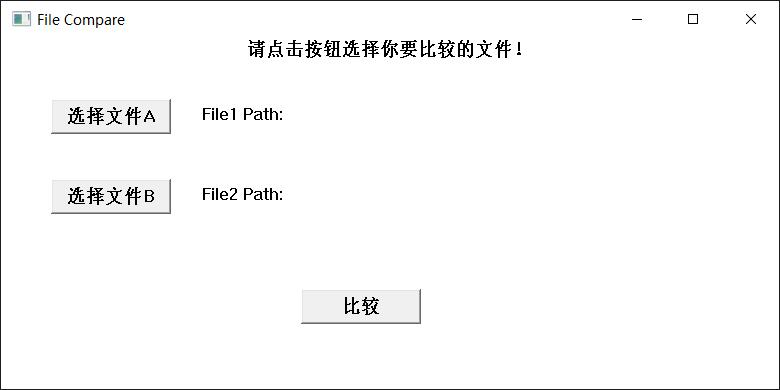
\includegraphics[width= 0.9\textwidth]{assets/界面设计}
    \caption{界面设计}
    \label{界面设计}
\end{figure}

\subsection{程序流程}
\begin{enumerate}
    \item 建立窗口显示界面,同时循环监听消息
    \item 点击选择文件后,打开选择文件对话框,同时得到相应的文件路径名
    \item 打开相应文件路径,读取文件内容,一行一行比对,得出结果
    \item 得到结果后,弹出窗口显示
\end{enumerate}

\section{具体实现}
该节介绍了代码中的部分核心算法和具体代码,包括了建立窗口,选择文件,文件对比,显示结果。

\subsection{建立窗口}
创建窗口,同时显示一系列信息到界面上。

流程如下:
\begin{enumerate}
    \item 获得当前程序的句柄;
    \item 注册窗口;
    \item 建立并显示窗口;
    \item 之后不断监听消息。
\end{enumerate}

具体代码如下:
\begin{lstlisting}
_WinMain	proc	
    local @stWndClass:WNDCLASSEX
    local @stMsg:MSG

    invoke GetModuleHandle,NULL		
    ;获得当前程序的句柄
    mov hInstance,eax
    invoke RtlZeroMemory,addr @stWndClass,sizeof @stWndClass

    ;注册窗口
    invoke LoadCursor,0,IDC_ARROW
    mov @stWndClass.hCursor,eax
    push hInstance
    pop @stWndClass.hInstance
    mov @stWndClass.cbSize, sizeof WNDCLASSEX			
    mov @stWndClass.style, CS_HREDRAW or CS_VREDRAW
    mov @stWndClass.lpfnWndProc,offset _ProcWinMain	
    ;过程地址		
    mov @stWndClass.hbrBackground, COLOR_WINDOW+1			
    mov @stWndClass.lpszClassName, offset szClassName		
    invoke RegisterClassEx, addr @stWndClass

    ;建立并显示窗口
    invoke CreateWindowEx, WS_EX_CLIENTEDGE,\  
                   offset szClassName, offset szCaptionMain,\  
                   WS_OVERLAPPEDWINDOW, \
                   300, 200, 800, 400,\	
                   NULL, NULL, hInstance, NULL
    mov hWinMain, eax										
    ;保存窗口句柄
    invoke ShowWindow, hWinMain, SW_SHOWNORMAL				 
    ;显示窗口		
    invoke UpdateWindow, hWinMain							
    ;绘制客户区
    
    ;消息循环
    .while TRUE
        invoke GetMessage,addr @stMsg,NULL,0,0
        .break .if eax == 0		
        ;如果是WM_QUIT,则结束循环
        invoke TranslateMessage,addr @stMsg
        invoke DispatchMessage,ADDR @stMsg
        .endw
        ret
_WinMain endp
\end{lstlisting}

\subsection{窗口过程函数}
循环监听消息,对于收到不同的消息,程序处理的函数不一样。

流程如下:
\begin{enumerate}
\item WM\_PAINT:表示绘制窗口的时候,需要执行的动作,展示窗口的一些提示信息;
\item WM\_CREATED:窗口接收到创建消息时,创建按钮和文本框;
\item WM\_COMMAND:根据eax的不同,分别执行不同的函数;
    \iitem eax==1或eax==2:打开文本对话框,将选择文件路径保存到filepath中;
    \iitem eax==3:进行文件比对,并弹出结果信息(注意输出行号的时候要转化成字符串形式)。
\end{enumerate}

具体代码如下:

\begin{lstlisting}
;窗口句柄,消息标识,消息参数
_ProcWinMain proc uses ebx edi esi, 
    hWnd, uMsg, wParam, lParam		
    local @stPs:PAINTSTRUCT
    local @stRect:RECT
    local @hDc
    local @temp:dword
    local @buffer[1024]:byte
    local @TextMSG[1024]:byte
    mov eax,uMsg


.if eax==WM_PAINT
    ;获取窗口设备环境句柄
    invoke BeginPaint, hWnd, addr @stPs			
    mov @hDc, eax					
    
    ;获取客户区大小
    invoke GetClientRect,hWnd,addr @stRect		
    invoke DrawText,@hDc,addr szText,-1,\
            addr @stRect,\
            DT_CENTER
    invoke	lstrlen, offset textout1
    invoke TextOut,@hDc, 200,65,offset textout1,eax
    invoke	lstrlen, offset textout2
    invoke TextOut,@hDc, 200,145,offset textout2,eax
    invoke EndPaint, hWnd, addr @stPs

;窗口关闭消息
.elseif eax==WM_CLOSE  
    invoke DestroyWindow, hWinMain
    ;发出WM_QUIT消息来退出循环
    invoke PostQuitMessage, NULL	


.elseif eax==WM_CREATE 
    invoke CreateWindowEx,NULL,\
            offset szbutton,offset button1,\
            WS_CHILD OR WS_VISIBLE,\
            50,60,120,35,\
            hWnd,1,hInstance,NULL

    invoke CreateWindowEx,NULL,\
            offset szbutton,offset button2,\
            WS_CHILD OR WS_VISIBLE,\
            50,140,120,35,\
            hWnd,2,hInstance,NULL

    invoke CreateWindowEx,NULL,\
            offset szbutton,offset button3,\
            WS_CHILD OR WS_VISIBLE,\
            300,250,120,35,\
            hWnd,3,hInstance,NULL

    invoke CreateWindowEx,NULL,\
            offset szedit,NULL,\
            WS_CHILD OR WS_VISIBLE,\
            300,65,400,35,\
            hWnd,4,hInstance,NULL

    invoke CreateWindowEx,NULL,\
            offset szedit,NULL,\
            WS_CHILD OR WS_VISIBLE,\
            300,145,400,35,\
            hWnd,5,hInstance,NULL

.elseif eax==WM_COMMAND
    mov eax,wParam
    .if eax == 1
        invoke OpenFileDirectory ,offset filePath1				;打开文件对话框选中相应文件
        invoke  SetDlgItemText, hWnd, 4, offset filePath1		;输出相应的文件路径到窗口上
    .elseif eax == 2
        invoke OpenFileDirectory ,offset filePath2
        invoke  SetDlgItemText, hWnd, 5, offset filePath2
    .elseif eax == 3
        invoke CompareFile ,offset filePath1,offset filePath2
        .if lineCount==0
        invoke  MessageBoxA, NULL, offset output1,
                offset szBoxTitle, MB_OK+MB_ICONINFORMATION
        .elseif
            xor esi,esi
            pusha
                invoke crt_strcat,addr @TextMSG,offset output2
            popa
            .while esi < lineCount
                mov edi,lineSeqs[esi*4]
                mov @temp,edi
                pusha
                invoke crt_sprintf ,addr @buffer,addr testout,@temp
                popa
                invoke crt_strcat,addr @TextMSG,addr @buffer
                inc esi
            .endw
            
            invoke  MessageBoxA, NULL, addr @TextMSG,
                offset szBoxTitle, MB_OK+MB_ICONERROR
        .endif
    .endif 

;其他默认一部分的消息
.else
    invoke DefWindowProc,hWnd,uMsg,wParam,lParam
    ret
.endif
xor eax,eax
ret

_ProcWinMain endp    
\end{lstlisting}

\subsection{文件对比}
将得到数组中的每一个元素对应相乘再相加。

流程如下:
\begin{enumerate}
   \item 打开文件,获得文件句柄;
   \item 不断循环,直到到达文件的末尾为止;
   \item 循环体内一行一行读取文件内容(crt\_fgets),并进行比对;
   \iitem 先判断长度是否相同,不相同则一定不等
   \iitem 若长度相同,则进一步比对内容(lstrcmp),并保存结果 
\end{enumerate}


具体代码如下:
\begin{lstlisting}
CompareFile proc stdcall, path1:ptr byte,path2:ptr byte
	local @pfile1:ptr FILE
	local @pfile2:ptr FILE
	local @readnum
	local @temp1,@temp2
	local @len1,@len2
	local @idx
	
	;打开文件
	invoke crt_fopen ,path1,offset textOpenPermisson	
	mov @pfile1,eax

	invoke crt_fopen,path2,offset textOpenPermisson
	mov @pfile2,eax

	mov @idx,0
	
	.while TRUE

		inc @idx
		mov @len1,0
		mov @len2,0
		mov @temp1,1
		mov @temp2,1

        ;初始化缓冲区
		invoke crt_memset, addr data1, 0, sizeof data1		
		invoke crt_memset, addr data2, 0, sizeof data2
		
		invoke crt_feof, @pfile1
		mov @temp1,eax
		invoke crt_feof, @pfile2
		mov @temp2,eax

		mov ecx,@temp1
		mov edx,@temp2
		.break .if ecx && edx

        ;说明没有到文件末尾
		.if !@temp1											
			invoke crt_fgets ,addr data1,1024,@pfile1
			invoke lstrlen,addr data1
			mov @len1,eax	
		.endif

		.if !@temp2
			invoke crt_fgets ,addr data2,1024,@pfile2
			invoke lstrlen,addr data2
			mov @len2,eax
		.endif
		

		mov eax,@len1
		mov ebx,@len2
		.if eax!=ebx							
		    ;长度不等当然不一样		
			mov ecx,lineCount	
			mov ebx,@idx
			lea esi,lineSeqs
			mov [esi+ecx*4],ebx
			inc lineCount
			.continue
		.endif
				
		invoke lstrcmp,addr data1,addr data2
		mov @temp1,eax
		
		.if eax			
			mov ecx,lineCount
			mov ebx,@idx
			lea esi,lineSeqs
			mov [esi+ecx*4],ebx
			inc lineCount			
		.endif

	.endw
	ret

CompareFile endp
\end{lstlisting}


\section{实验结果展示}

\subsection{两个文件相同}
\begin{figure}[H]
    \centering
    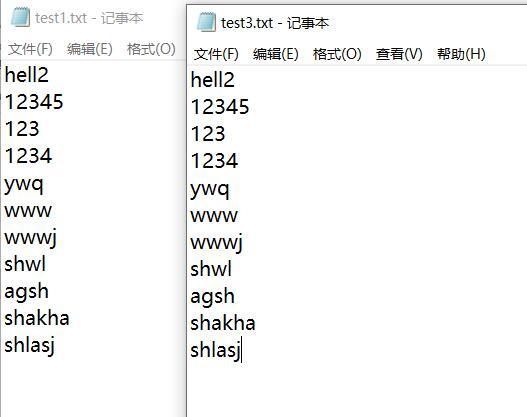
\includegraphics[width= 0.9\textwidth]{assets/文件比对3}
    \caption{文件内容相同}
    \label{文件内容3}
\end{figure}
\begin{figure}[H]
    \centering
    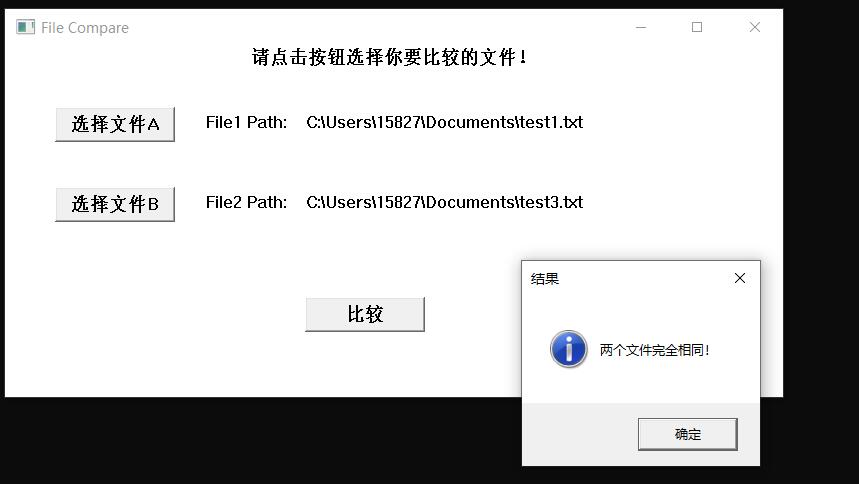
\includegraphics[width= 0.9\textwidth]{assets/文件比对4}
    \caption{文件比对结果}
    \label{文件比对结果1}
\end{figure}
\subsection{两个文件内容不同}
\begin{figure}[H]
    \centering
    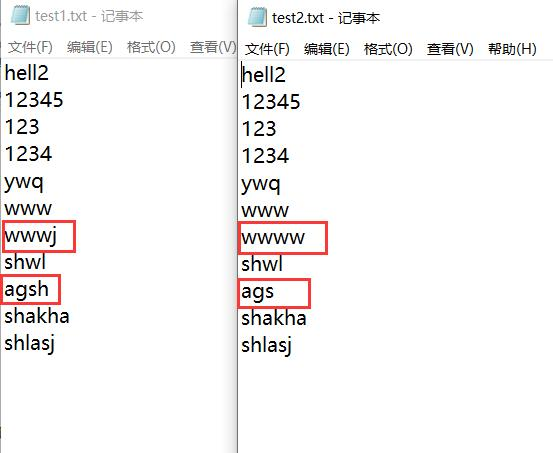
\includegraphics[width= 0.9\textwidth]{assets/文件比对2}
    \caption{文件内容不同}
    \label{文件内容不同}
\end{figure}
\begin{figure}[H]
    \centering
    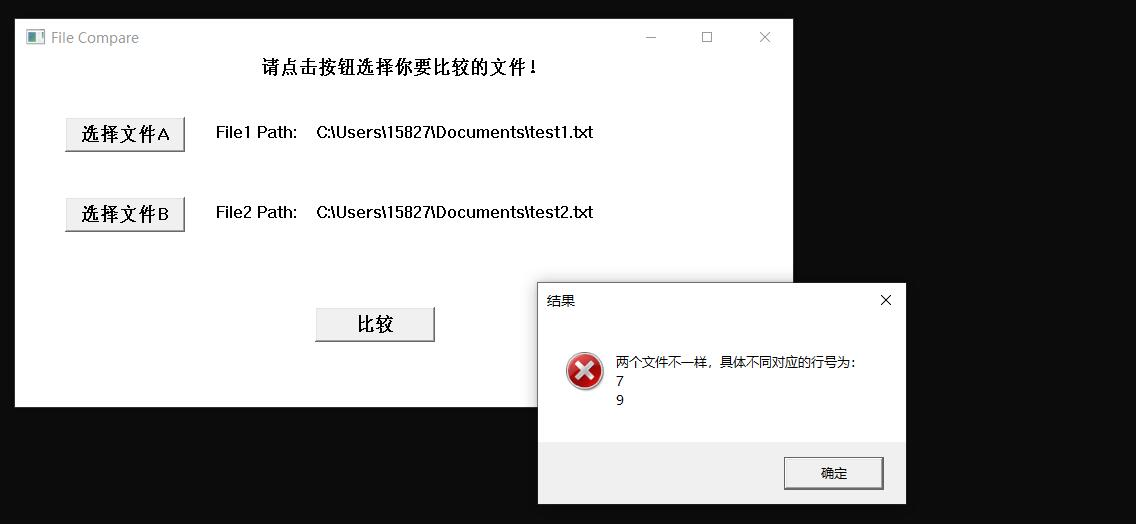
\includegraphics[width= 0.9\textwidth]{assets/文件对比1}
    \caption{文件比对结果}
    \label{文件比对结果2}
\end{figure}

